\documentclass[a4paper]{article}
\newcounter{QuestionNumber}
\setcounter{QuestionNumber}{1}

\newcommand{\Q}{
\textbf{Question \theQuestionNumber)}
\stepcounter{QuestionNumber}
}
\usepackage{amsmath,amssymb,graphicx,subcaption,caption}
\usepackage{enumitem}
\usepackage[margin=1in]{geometry}
\usepackage{lipsum}
 \renewcommand{\familydefault}{\rmdefault}
\setlength{\parindent}{0pt}
\setlength{\parskip}{1em}
\begin{document}
\Large
\begin{center}
In the name of beauty

The 11th problem set solution of Optical Networks course

\hrulefill
\end{center}

\Q

\begin{enumerate}[label=\alph*-]
\item
Path restoration requires a link-and-node-disjoint path with respect to the working path. Such a path could be 1-3-6-8 with 3 hops.
\item
We protect the segment 2-5-8 of the working path through the segment 2-6-8, with 3 hops in total.
\item
Link protection is more local to the other two. It only concerns protecting a single link and generates the path 1-2-6-5-8 as the backup with 4 hops. Such a methodology may lead to extra hops.
\end{enumerate}

\Q

The event that the back-up path would be sufficient, is equivalent to at most one working path be brought down simultaneously. Its probability is
$$
\hat P=\sum_{k=0}^1\binom{n}{k}(1-p)^kp^{n-k}
=p^n+np^{n-1}(1-p),
$$
hence, the desired probability is
$$
P=1-\hat P=1-p^n-np^{n-1}(1-p).
$$

\Q

We solve this question by calculating the number of cases where the connection does not survive from a double-link failure. In this case, it is intuitive that one link must be down on each (working and protection) path. Since the two paths of the connection have 4 and 5 links, the total number of outcomes such that the connection cannot survive, is equal to $4\times 5=20$. Hence, the connection survives in
$
\binom{11}{2}-20=35
$
ways (the term $\binom{11}{2}$ stands for the total number of double-link failure events). 

\Q

When protection is deployed to protect a connection, both paths must have the same wavelength. To consider this constraint in our graph-coloring problem for WA, we must set this regulation that \textit{two connections coincide if and only if either one of their working or protections paths do}. Enumerating the routed connections by 1 to 6 from above, the conflict graph would be

\begin{figure}[h]
\centering
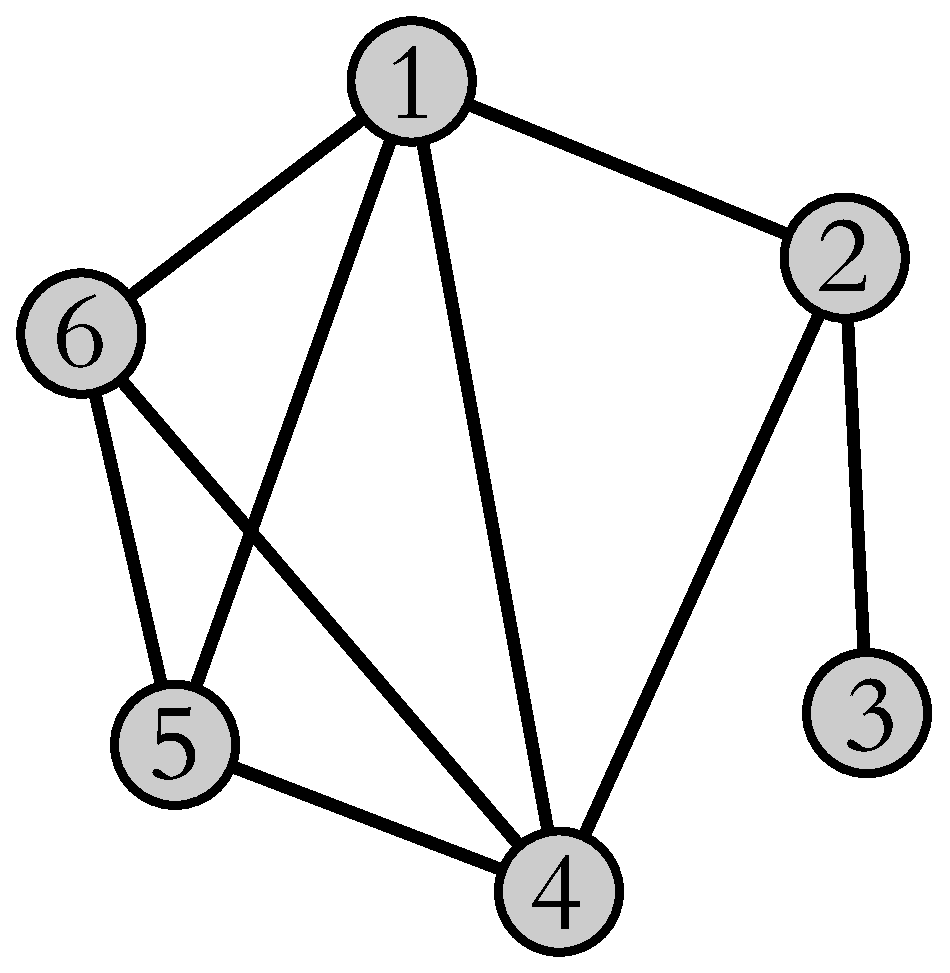
\includegraphics[width=50mm]{con_gr_prot.eps}
\end{figure}

Using the first-fit heuristics, we obtain

\begin{table}[h]
\Large
\centering
\begin{tabular}{|c|c|}
\hline
Connection Number&Assigned Wavelength
\\\hline
1&$\lambda_1$
\\\hline
2&$\lambda_2$
\\\hline
3&$\lambda_1$
\\\hline
4&$\lambda_3$
\\\hline
5&$\lambda_2$
\\\hline
6&$\lambda_4$
\\\hline
\end{tabular}
\end{table}

\end{document}


